% Created 2022-09-15 jue 12:36
% Intended LaTeX compiler: pdflatex
\documentclass[12pt]{article}
\usepackage[utf8]{inputenc}
\usepackage[T1]{fontenc}
\usepackage{graphicx}
\usepackage{grffile}
\usepackage{longtable}
\usepackage{wrapfig}
\usepackage{rotating}
\usepackage[normalem]{ulem}
\usepackage{amsmath}
\usepackage{textcomp}
\usepackage{amssymb}
\usepackage{capt-of}
\usepackage{hyperref}
\usepackage[spanish]{babel}
\usepackage{graphicx,geometry}
\geometry{ a4paper, left=1in, right=1in, top=1in, bottom=1in }
\renewcommand\familydefault{\sfdefault}
\usepackage{sectsty}
\sectionfont{\normalfont\Large }
\subsectionfont{\normalfont\normalsize}
\usepackage{tabularx}
\usepackage{listings}
\lstdefinestyle{mystyle}{
numbers=left,
showspaces=false,
frame=leftline,
showspaces=false,
showstringspaces=false,
showtabs=false,
numberstyle=\tiny,
}
\lstset{
style=mystyle,
literate={á}{{\'a}}1
{é}{{\'e}}1
{í}{{\'{\i}}}1
{ó}{{\'o}}1
{ú}{{\'u}}1
{Á}{{\'A}}1
{É}{{\'E}}1
{Í}{{\'I}}1
{Ó}{{\'O}}1
{Ú}{{\'U}}1
{ü}{{\"u}}1
{Ü}{{\"U}}1
{ñ}{{\~n}}1
{Ñ}{{\~N}}1
{¿}{{?``}}1
{¡}{{!``}}1
}
\makeatletter
\usepackage{fancyhdr}
\pagestyle{fancy}
\usepackage{mdframed}
\BeforeBeginEnvironment{minted}{\begin{mdframed}}
\AfterEndEnvironment{minted}{\end{mdframed}}
\author{Luis Eduardo Galindo Amaya (1274895)}
\date{2022-09-15}
\title{Regrecion Lineal}
\hypersetup{
 pdfauthor={Luis Eduardo Galindo Amaya (1274895)},
 pdftitle={Regrecion Lineal},
 pdfkeywords={},
 pdfsubject={},
 pdfcreator={Emacs 26.3 (Org mode 9.1.9)}, 
 pdflang={Spanish}}
\begin{document}


\newcommand{\docente}{Olivia Mendoza Duarte}
\newcommand{\asignatura}{Estadística Avanzada}
\newcommand{\semestre}{2022-2}

\newcommand{\miportada}[1]{
	\begin{titlepage}
		\vspace*{0.75in}
		\begin{flushleft}
			\sffamily
			\large #1       \\
			\Huge
            \@title         \\
			\hrulefill
			\vspace{0.25in} \\
			\Large \@author \\
			\vspace*{\fill}
            
\includegraphics[width=\textwidth]{../includes/filler.png} \\
			\vspace*{\fill}
			\large
			\begin{tabular}{|l|l|}
              \hline
			  Asignatura & \asignatura \\
			  Docente    & \docente    \\
			  Fecha      & \@date      \\
              \hline
			\end{tabular}
		\end{flushleft}
	\end{titlepage}
}

\miportada{ Práctica }

\fancyhf{}
\lhead{ \asignatura }
\rhead{ \semestre }
\rfoot{Página \thepage}

\setlength\parindent{0pt}   % eliminar el intentado
\setlength{\parskip}{1.2em}

\maketitle
\end{center}

\section*{Bicis Por Dia - Temp}
\label{sec:org516b60e}
\subsection*{prompt}
\label{sec:org3277e9d}
\begin{verbatim}
=== Classifier model (full training set) ===

Linear regression on temp
173.71 * temp + 279.95

Predicting 0 if attribute value is missing.
Time taken to build model: 0 seconds

=== Cross-validation ===
=== Summary ===

Correlation coefficient                  0.1338
Mean absolute error                    182.9304
Root mean squared error                209.1587
Relative absolute error                 99.9184 %
Root relative squared error             98.979  %
Total Number of Instances              731     
\end{verbatim}

\subsection*{captura}
\label{sec:orgce4ef83}
\begin{center}
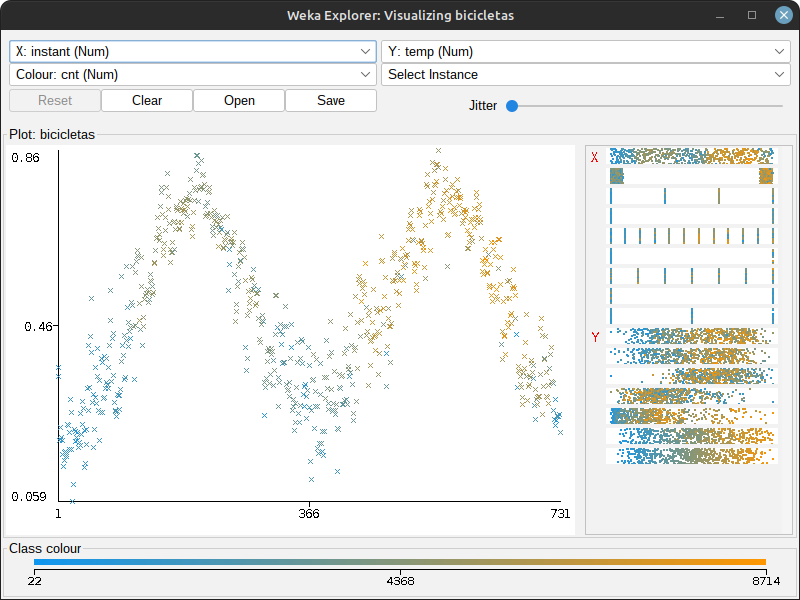
\includegraphics[width=10cm]{img/grafica-bicis-dia-temp.png}
\end{center}

\section*{Bicis por Hora - Temp}
\label{sec:org86b8e99}
\subsection*{Prompt}
\label{sec:orgaa072cd}
\begin{verbatim}
=== Classifier model (full training set) ===

Linear regression on temp

3548.1 * temp + 6926.64

Predicting 0 if attribute value is missing.
Time taken to build model: 0 seconds

=== Cross-validation ===
=== Summary ===
Correlation coefficient                  0.1355
Mean absolute error                   4340.2185
Root mean squared error               4970.6098
Relative absolute error                 99.8908 %
Root relative squared error             99.0728 %
Total Number of Instances            17379     
\end{verbatim}

\subsection*{Captura}
\label{sec:orgd4cb78d}
\begin{center}
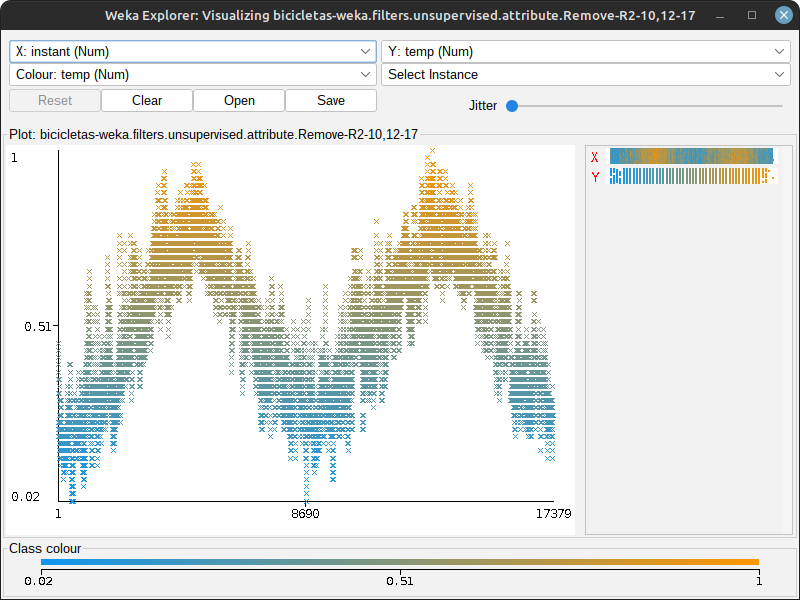
\includegraphics[width=10cm]{img/2.png}
\end{center}

\section*{Gruas - Angle}
\label{sec:org05a0705}
\subsection*{prompt}
\label{sec:org003faa5}
\begin{verbatim}
=== Classifier model (full training set) ===

Linear regression on Speed

0.07 * Speed - 0.38

Predicting 0 if attribute value is missing.
Time taken to build model: 0 seconds

=== Cross-validation ===
=== Summary ===

Correlation coefficient                 -0.6982
Mean absolute error                      3.3747
Root mean squared error                  4.0533
Relative absolute error                111.6984 %
Root relative squared error            111.0355 %
Total Number of Instances               15     
\end{verbatim}

\subsection*{Captura}
\label{sec:org5d5a067}
\begin{center}
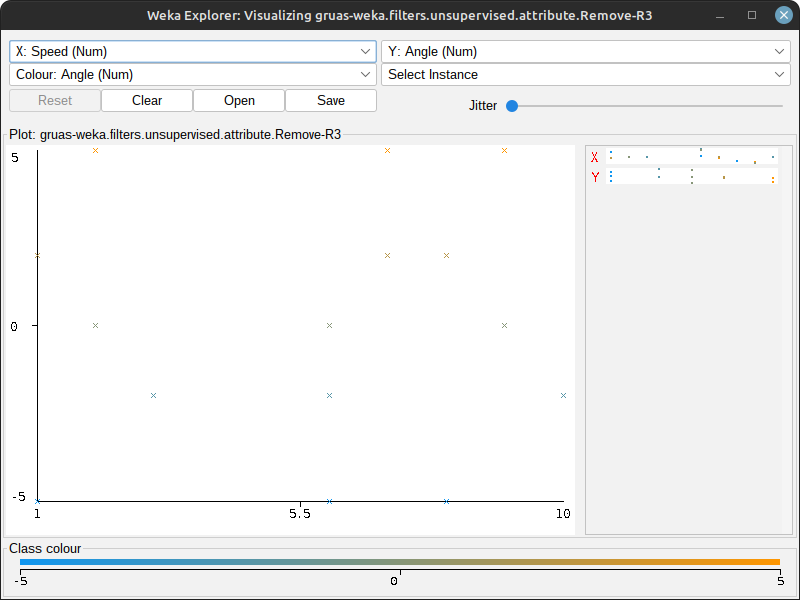
\includegraphics[width=10cm]{img/3.png}
\end{center}

\section*{Código para regrecion linel simple en R}
\label{sec:orgb59d6b9}
\begin{verbatim}
## Eje x
x = c(1:10)
## Eje Y
y = c(34, 36, 19, 20, 22, 20, 19, 13, 15, 16)
n = length(y)

if( length(y) != length(x) ) {
    stop("Los arreglos son de simenciones diferentes")
}

## multiplicacion de elementos
xy = x*y

## elementos al cuadrado
xp2 = x^2

## pendiente 
m = (n * sum(xy) - sum(x)*sum(y))/(n*sum(xp2) - sum(xp2))

## ordenada de origen
b = (sum(y) - m*sum(x))/n

## termina
print(sprintf("%fx + %f", m, b))
\end{verbatim}
\end{document}
